Targeted users are users who would use Magpie as a tool for their work. We interviewed 3 individuals who fit this criteria.\\ \\
Usability test sessions took the following format:
\begin{enumerate}
    \item Getting to know
    \item Introduction of Magpie
    \item Exploring Magpie + Discussion
    \item Satisfaction survey + End of session
\end{enumerate}
Getting to know the professional user is the first step. It is relevant to the session because it helps inform the type of targeted user they are, their knowledge of technology, their experience using amenity data, the tools they have used and their perspective regarding amenities.

\subsubsection{User 7 - Bryan Boyle}
Bryan Boyle is a lecturer at the University of Cork in Occupational sciences and Therapy.\\ With a doctorate in computer science and occupational therapy, they have published several papers related to inclusivity in public spaces (\cite{bryanboyleplaygroundinclusion2023}), and the role of technology in the lives of individuals with disabilities (\cite{bryanboylechildrenautism2022}).\\ \\
They left their contact in the market research survey. They are categorized as a \emph{targeted user} because they use amenity data for their work, and Magpie could potentially be a tool they use.\\

\noindent Firstly, we got to know Bryan Boyle, his professional experience and the amenity data he uses for his work.\\
He is mostly into research and therefore looks for datasets related to PHD topics of child development and inclusivity.
%bryan amenity info
\begin{figure}[h!]
    \centering
    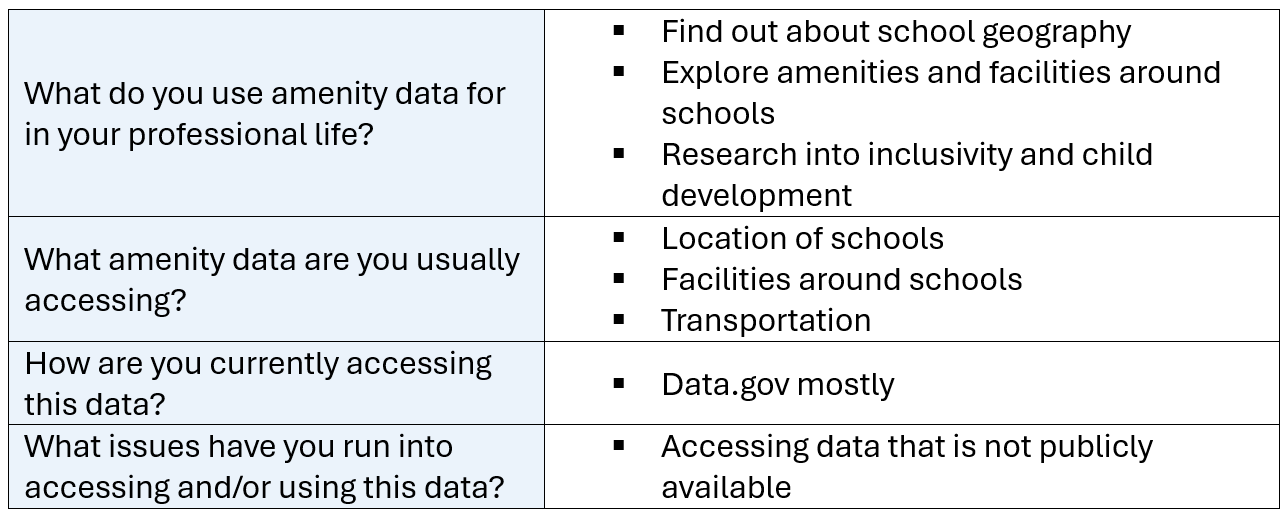
\includegraphics[width=0.9\textwidth]{images/bryan-amenity-info.png}
    \caption{User Evaluation - Bryan Boyle Information}
\end{figure}\\

\noindent Next, we introduced Magpie and started the uncontrolled session.\\
The approach was to guide Bryan Boyle through the homepage whilst introducing Magpie, and then let them roam around on their own while discussing his their thoughts. They were able to complete most of the general tasks, except for zooming in and out. This is because they were not familiar with mouse technology, the onboarding was not clear enough and zoom buttons were not present on the map.
%table of Bryan's general tasks
\begin{table}[h!]
    \centering
    \caption{Usability testing Tasks - Bryan}
    \begin{tabular}{|p{0.4\textwidth}|p{0.1\textwidth}|p{0.1\textwidth}|p{0.1\textwidth}|p{0.1\textwidth}|}
        \hline
        \textbf{Task}                 & \textbf{Status} & \textbf{Difficulty} & \textbf{Errors} \\
        \hline
        Load Magpie application       & Complete        & 2                   & N/A             \\
        \hline
        Sign up                       & Complete        & 1                   & N/A             \\
        \hline
        Log in                        & Complete        & 1                   & N/A             \\
        \hline
        Complete tutorial             & Complete        & 1                   & N/A             \\
        \hline
        Place cursor on map           & Pass            & 3                   & Required help   \\
        \hline
        Zoom in and out               & Fail            & 5                   & Required help   \\
        \hline
        Hold map and navigate         & Complete        & 1                   & N/A             \\
        \hline
        Adjust radius big/small       & Complete        & 1                   & N/A             \\
        \hline
        Clear marker \& radius        & Complete        & 2                   & N/A             \\
        \hline
        Deselect all amenities        & Complete        & 2                   & N/A             \\
        \hline
        Select one or more amenities  & Complete        & 1                   & N/A             \\
        \hline
        Find tutorial and exit midway & Complete        & 2                   & N/A             \\
        \hline
        Log out                       & Complete        & 1                   & N/A             \\
        \hline
    \end{tabular}
\end{table}\\
\newpage Here were the main takeaways from Bryan's session:
\begin{itemize}
    \item \textbf{Data: }they mainly looked at amenities related to accessibility such as accessible parking, public toilets, water fountains, etc... They would like to see more data such as public transportation, public facilities like schools, hospitals and stations.\\ What really interests them is the type and quality of an amenity surrounding the specific location they are searching for, so this would require more higher-level information to add to the tooltips.\\
    \item \textbf{General: }they really enjoyed using the search bar, they found it intuitive and quicker to use than placing a marker directly on the map. They are very interested in the project and look forward to seeing the final product.\\
    \item \textbf{Behaviour: } Bryan seems to not be very comfortable with technology. Throughout the session, we noticed that first they used Edge as a browser, they got lost looking for the tab among the many windows they had open, their browser window was not full screen and additionally struggled zooming into the map.
\end{itemize}
The survey answers below complement his vocal feedback:
\fcolorbox{yellow}{yellow}{BRYAN SURVEY RESPONSES}\\

\textbf{Overall}, Bryan found Magpie to be nice, simple and very straightforward. He would use it as a tool for his PHD research, mainly on desktop which further solidifies our user persona and why we prioritized desktop compatibility before mobile.

\newpage
\subsubsection{User 8 - Anonymous}
Professional user Sarah

\newpage
\subsubsection{User 9 - Anonymous}
Professional user Odran